\documentclass[14pt]{beamer}
\usepackage[T2A]{fontenc}
\usepackage[utf8]{inputenc}
\usepackage[english,russian]{babel}
\usepackage{amssymb,amsfonts,amsmath,mathtext}
\usepackage{cite,enumerate,float,indentfirst}

%\usepackage{CJKutf8}

\graphicspath{{images/}}

\usetheme{Pittsburgh}
\usecolortheme{whale}

\setbeamercolor{footline}{fg=blue}
\setbeamertemplate{footline}{
  \leavevmode%
  \hbox{%
  \begin{beamercolorbox}[wd=.333333\paperwidth,ht=2.25ex,dp=1ex,center]{}%
    Куликов А.В., ABBYY-MIPT
  \end{beamercolorbox}%
  \begin{beamercolorbox}[wd=.333333\paperwidth,ht=2.25ex,dp=1ex,center]{}%
    Москва, 2016
  \end{beamercolorbox}%
  \begin{beamercolorbox}[wd=.333333\paperwidth,ht=2.25ex,dp=1ex,right]{}%
  Стр. \insertframenumber{} из \inserttotalframenumber \hspace*{2ex}
  \end{beamercolorbox}}%
  \vskip0pt%
}

\newcommand{\itemi}{\item[\checkmark]}

\title{\small{Японский: буквенные n-граммы для распознавания}}
\subtitle{\footnotesize{Контроль НИР}}
\author{\small{%
~Куликов А.В., гр. 397\\%
\emph{Руководитель:}~Андрианов А.И.}\\%
\vspace{30pt}%
ABBYY-MIPT%
\vspace{20pt}%
}
\date{\small{Москва, 2016}}

\begin{document}

\maketitle

\begin{frame}

\frametitle{Задача}
\begin{itemize}
    \item Japanese kanji/kana OCR.
    \item Существуют путающиеся символы, например:
    \begin{figure}[h]
        \center{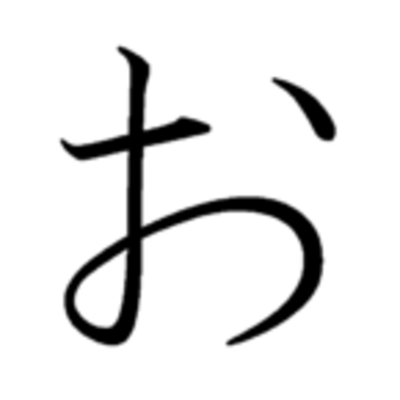
\includegraphics[scale=0.05]{KanaO}\ и 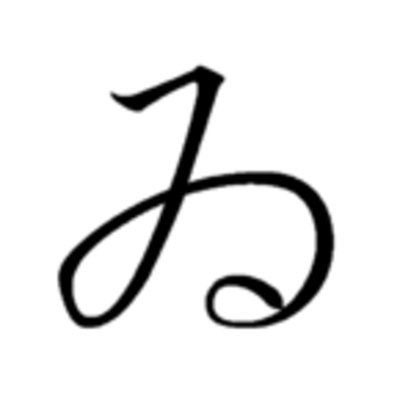
\includegraphics[scale=0.05]{KanaWi}}
    \end{figure}
    \item \emph{Цель работы: } построить систему исправления ошибок OCR, используя буквенную n-граммную модель языка.
\end{itemize}
\end{frame}

\begin{frame}
\frametitle{Что нужно сделать?}
\begin{itemize}
    \item Выучить японский;
    \item Изучить имеющиеся подходы к задаче;
    \item Понять суть используемых методов и алгоритмов;
    \item Выбрать корпуса для тестирования;
    \item Определить Baseline;
    \item Улучшать качество исправления.
\end{itemize}
\end{frame}

\begin{frame}
\frametitle{Что было сделано?}
\begin{itemize}
    \item Японский постепенно ботается;
    \item Был прочитан ряд статей по теме;
    \item Изучены возможности python-nltk;
    \item Найдены несколько корпусов (KOTOHONA, RWCP, EDR etc.);
    \item Сделаны прикидки для Baseline.
\end{itemize}
\end{frame}

\begin{frame}
\frametitle{Текущие результаты}
\begin{itemize}
  \item Знаю хирагану и ещё чуть-чуть;
  \item Markov chains, accuracy metric;
  \item На первых порах nltk более, чем достаточно;
  \item Были тестовые прогоны на небольших текстах.
\end{itemize}
\end{frame}

%\begin{frame}
%\frametitle{\begin{CJK}{UTF8}{min}
%日本 -- bigrams on wikipage
%\end{CJK}}

%\begin{figure}[h]
%    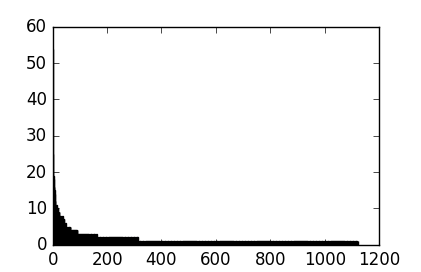
\includegraphics[scale=0.5]{nihon2}
%\end{figure}

%\center{
%\begin{CJK}{UTF8}{min}
%日本 --- 54 \\
%、日 --- 25 \\
%てい --- 19 \\
%は、 --- 18
%\end{CJK}
%}

%\end{frame}

\begin{frame}
\frametitle{Что делать дальше?}
\begin{itemize}
  \item Продолжать ботать японский;
  \item Прогоняться на корпусах, улучшая качество;
  \item Экспериментировать со сложными структурами (Hidden Markov Models, Conditional Random Fields etc.);
  \item Возможно, перейти на C для оптимизации.
\end{itemize}
\end{frame}

\begin{frame}
\frametitle{Список литературы}
\footnotesize{
\begin{itemize}
  \item Foundations of Statistical Natural Language Processing / \\C. D. Manning, H. Schutze.
  \item N-gram Language Modeling of Japanese Using Bunsetsu Boundaries / S. Chung, K. Hirose and N. Minematsu 
  \item Applying Conditional Random Fields to Japanese Morphological Analysis / T. Kudo, K. Yamamoto, Y. Matsumoto
  \item Survey of Pattern Recognition Approaches in Japanese Character Recognition / S. Das, S. Banerjee
\end{itemize}}
\end{frame}

%%%%%%%%%%%%%%%%%%%%%%%%%%%%%%

\begin{frame}

\center{\huge %\begin{CJK}{UTF8}{min}
%ありがとう
%\end{CJK}}
Спасибо!
}

\end{frame}

\end{document} 